%% NSS-MIC_Instructions.tex
%% 8/2007
%% By Bo Yu (yu@bnl.gov)
%% based on:
%% bare_jrnl.tex
%% V1.3
%% 2007/01/11
%% by Michael Shell
%% see http://www.michaelshell.org/
%% for current contact information.
%%
%% This is a skeleton file demonstrating the use of IEEEtran.cls
%% (requires IEEEtran.cls version 1.7 or later) with an IEEE journal paper.
%%
%% Support sites:
%% http://www.michaelshell.org/tex/ieeetran/
%% http://www.ctan.org/tex-archive/macros/latex/contrib/IEEEtran/
%% and
%% http://www.ieee.org/


%%*************************************************************************
%% Legal Notice:
%% This code is offered as-is without any warranty either expressed or
%% implied; without even the implied warranty of MERCHANTABILITY or
%% FITNESS FOR A PARTICULAR PURPOSE!
%% User assumes all risk.
%% In no event shall IEEE or any contributor to this code be liable for
%% any damages or losses, including, but not limited to, incidental,
%% consequential, or any other damages, resulting from the use or misuse
%% of any information contained here.
%%
%% All comments are the opinions of their respective authors and are not
%% necessarily endorsed by the IEEE.
%%
%% This work is distributed under the LaTeX Project Public License (LPPL)
%% ( http://www.latex-project.org/ ) version 1.3, and may be freely used,
%% distributed and modified. A copy of the LPPL, version 1.3, is included
%% in the base LaTeX documentation of all distributions of LaTeX released
%% 2003/12/01 or later.
%% Retain all contribution notices and credits.
%% ** Modified files should be clearly indicated as such, including  **
%% ** renaming them and changing author support contact information. **
%%
%% File list of work: IEEEtran.cls, IEEEtran_HOWTO.pdf, bare_adv.tex,
%%                    bare_conf.tex, bare_jrnl.tex, bare_jrnl_compsoc.tex
%%*************************************************************************
\documentclass[journal]{IEEEtran}
\usepackage{graphicx}

\begin{document}
\title{DQM4HEP : A generic\\Data Quality Monitoring for High Energy Physics}
%
% author names and IEEE memberships
% note positions of commas and nonbreaking spaces ( ~ ) LaTeX will not break
% a structure at a ~ so this keeps an author's name from being broken across
% two lines.
% use \thanks{} to gain access to the first footnote area
% a separate \thanks must be used for each paragraph as LaTeX2e's \thanks
% was not built to handle multiple paragraphs
%

\author{R. \'Et\'e, A. Pingault, L. Mirabito
\thanks{Manuscript received November 30, 2016.}% <-this % stops a space
\thanks{R. \'Et\'e is with Univ, Lyon, Universit\'e Lyon 1, CNRS/IN2P3, IPNL 4 rue E Fermi, 69622, Villeurbanne CEDEX, France (e-mail: rete@ipnl.in2p3.fr).}%
\thanks{A. Pingault is with Ghent University, Department of Physics and Astronomy Proeftuinstraat 86, B-9000 Gent, Belgium (e-mail: antoine.pingault@ugent.be).}%
\thanks{L. Mirabito is with Univ, Lyon, Universit\'e Lyon 1, CNRS/IN2P3, IPNL 4 rue E Fermi, 69622, Villeurbanne CEDEX, France (e-mail: mirabito@ipnl.in2p3.fr).}%
}

\maketitle
\pagestyle{empty}
\thispagestyle{empty}

\begin{abstract}
With increasingly sophisticated experiment, online Data Quality Monitoring (DQM) is of a significant importance for the detector and operation efficiency. Most experiments use their own Event Data Model (EDM) for data taking and built a dedicated monitoring system on top of it. This leads to a strong dependency to the data format and storage, making the reusability of the system for another experiment difficult.

To increase the flexibility and capabilities of software across experiments, we developed DQM4HEP, a generic online Data Quality Monitoring system specifically targeted to High Energy Physics experiments. The core principle was to make no assumption on the Event Data Model and data type to treat. The result provides reusable and flexible tools for scientists to monitor their detectors by focusing only on the data analysis part.

In addition, a dedicated implementation, based on the LCIO~\cite{LCIO} Event Data Model for the Linear Collider Collaboration (LCC), was also developed. It has already been put to real condition testing during test beam campaigns at CERN\footnote{Conseil Européen pour la Recherche Nucléaire} with a combined detector setup composed of the CALICE\footnote{CAlorimeter for LInear Collider Experiment} Semi-Digital Hadronic CALorimeter (SDHCAL) and Silicon Tungsten Electronic Calorimeter (SiWECal) prototypes.
\end{abstract}

\begin{IEEEkeywords}
DQM, HEP, Detector, DAQ.
\end{IEEEkeywords}

%\begin{IEEEkeywords}
%IEEEtran, journal, \LaTeX, paper, template.
%\end{IEEEkeywords}


\section{Introduction}
% The very first letter is a 2 line initial drop letter followed
% by the rest of the first word in caps.
%
% form to use if the first word consists of a single letter:
% \IEEEPARstart{A}{demo} file is ....
%
% form to use if you need the single drop letter followed by
% normal text (unknown if ever used by IEEE):
% \IEEEPARstart{A}{}demo file is ....
%
% Some journals put the first two words in caps:
% \IEEEPARstart{T}{his demo} file is ....
%
% Here we have the typical use of a "T" for an initial drop letter
% and "HIS" in caps to complete the first word.


\IEEEPARstart{T}{he} purpose of a monitoring system is to help the identification of problems when the experiment is running. For this, it needs to fulfill two requirements : it must display a quick overview of the status and working order of every detector part and should also evaluate the quality of the data being taken. This implies some key architecture points for the monitoring software. First, as it should be running at all times when taking data, it needs to interface with the Data Acquisition (DAQ) system. It must not however interfere with the data taking process (slow down, stop, etc.). It needs a system to distribute data coming from the DAQ to the analysis tools and then to visualization tools. The data analysis and data quality assessment needs to remain user-defined and visualization interfaces accessible from many client computers.

In computer science, generic programming implies an architecture with algorithms independent of a programming data type. Algorithms can be instantiated when needed, and in different ways to work with multiple data representations. This leads to more flexible and easily reusable software.

The genericity of the framework that is presented here, lies in two core features: its Event Data Model (EDM) abstraction and plugin system.

The EDM abstraction gives the ability to the user to define the type of event to use together with its serialization process. The plugin system, permits the inclusion of any user classes via external libraries. One can use plugin abstraction and factories to select the serialization process, online analysis, etc.

The framework is also designed to run each application as an independent process. Processes are linked to each other by network communications with either TCP/IP or HTTP protocols using DIM~\cite{DIM} and Mongoose~\cite{MONGOOSE} respectively. This helps distributing the load from the processes over multiple cores and computers.

To implement this solution for its own experiment, an user has to define the event type to treat and its serialization. An interface, \textit{xdrstream}, is provided within the framework to simplify the later.

\section{Software architecture}

The global framework architecture as seen on Fig.~\ref{fig:DQM4HEPArchitecture} is discussed in the following paragraphs.
\begin{figure}[htbp]
  \begin{center}
    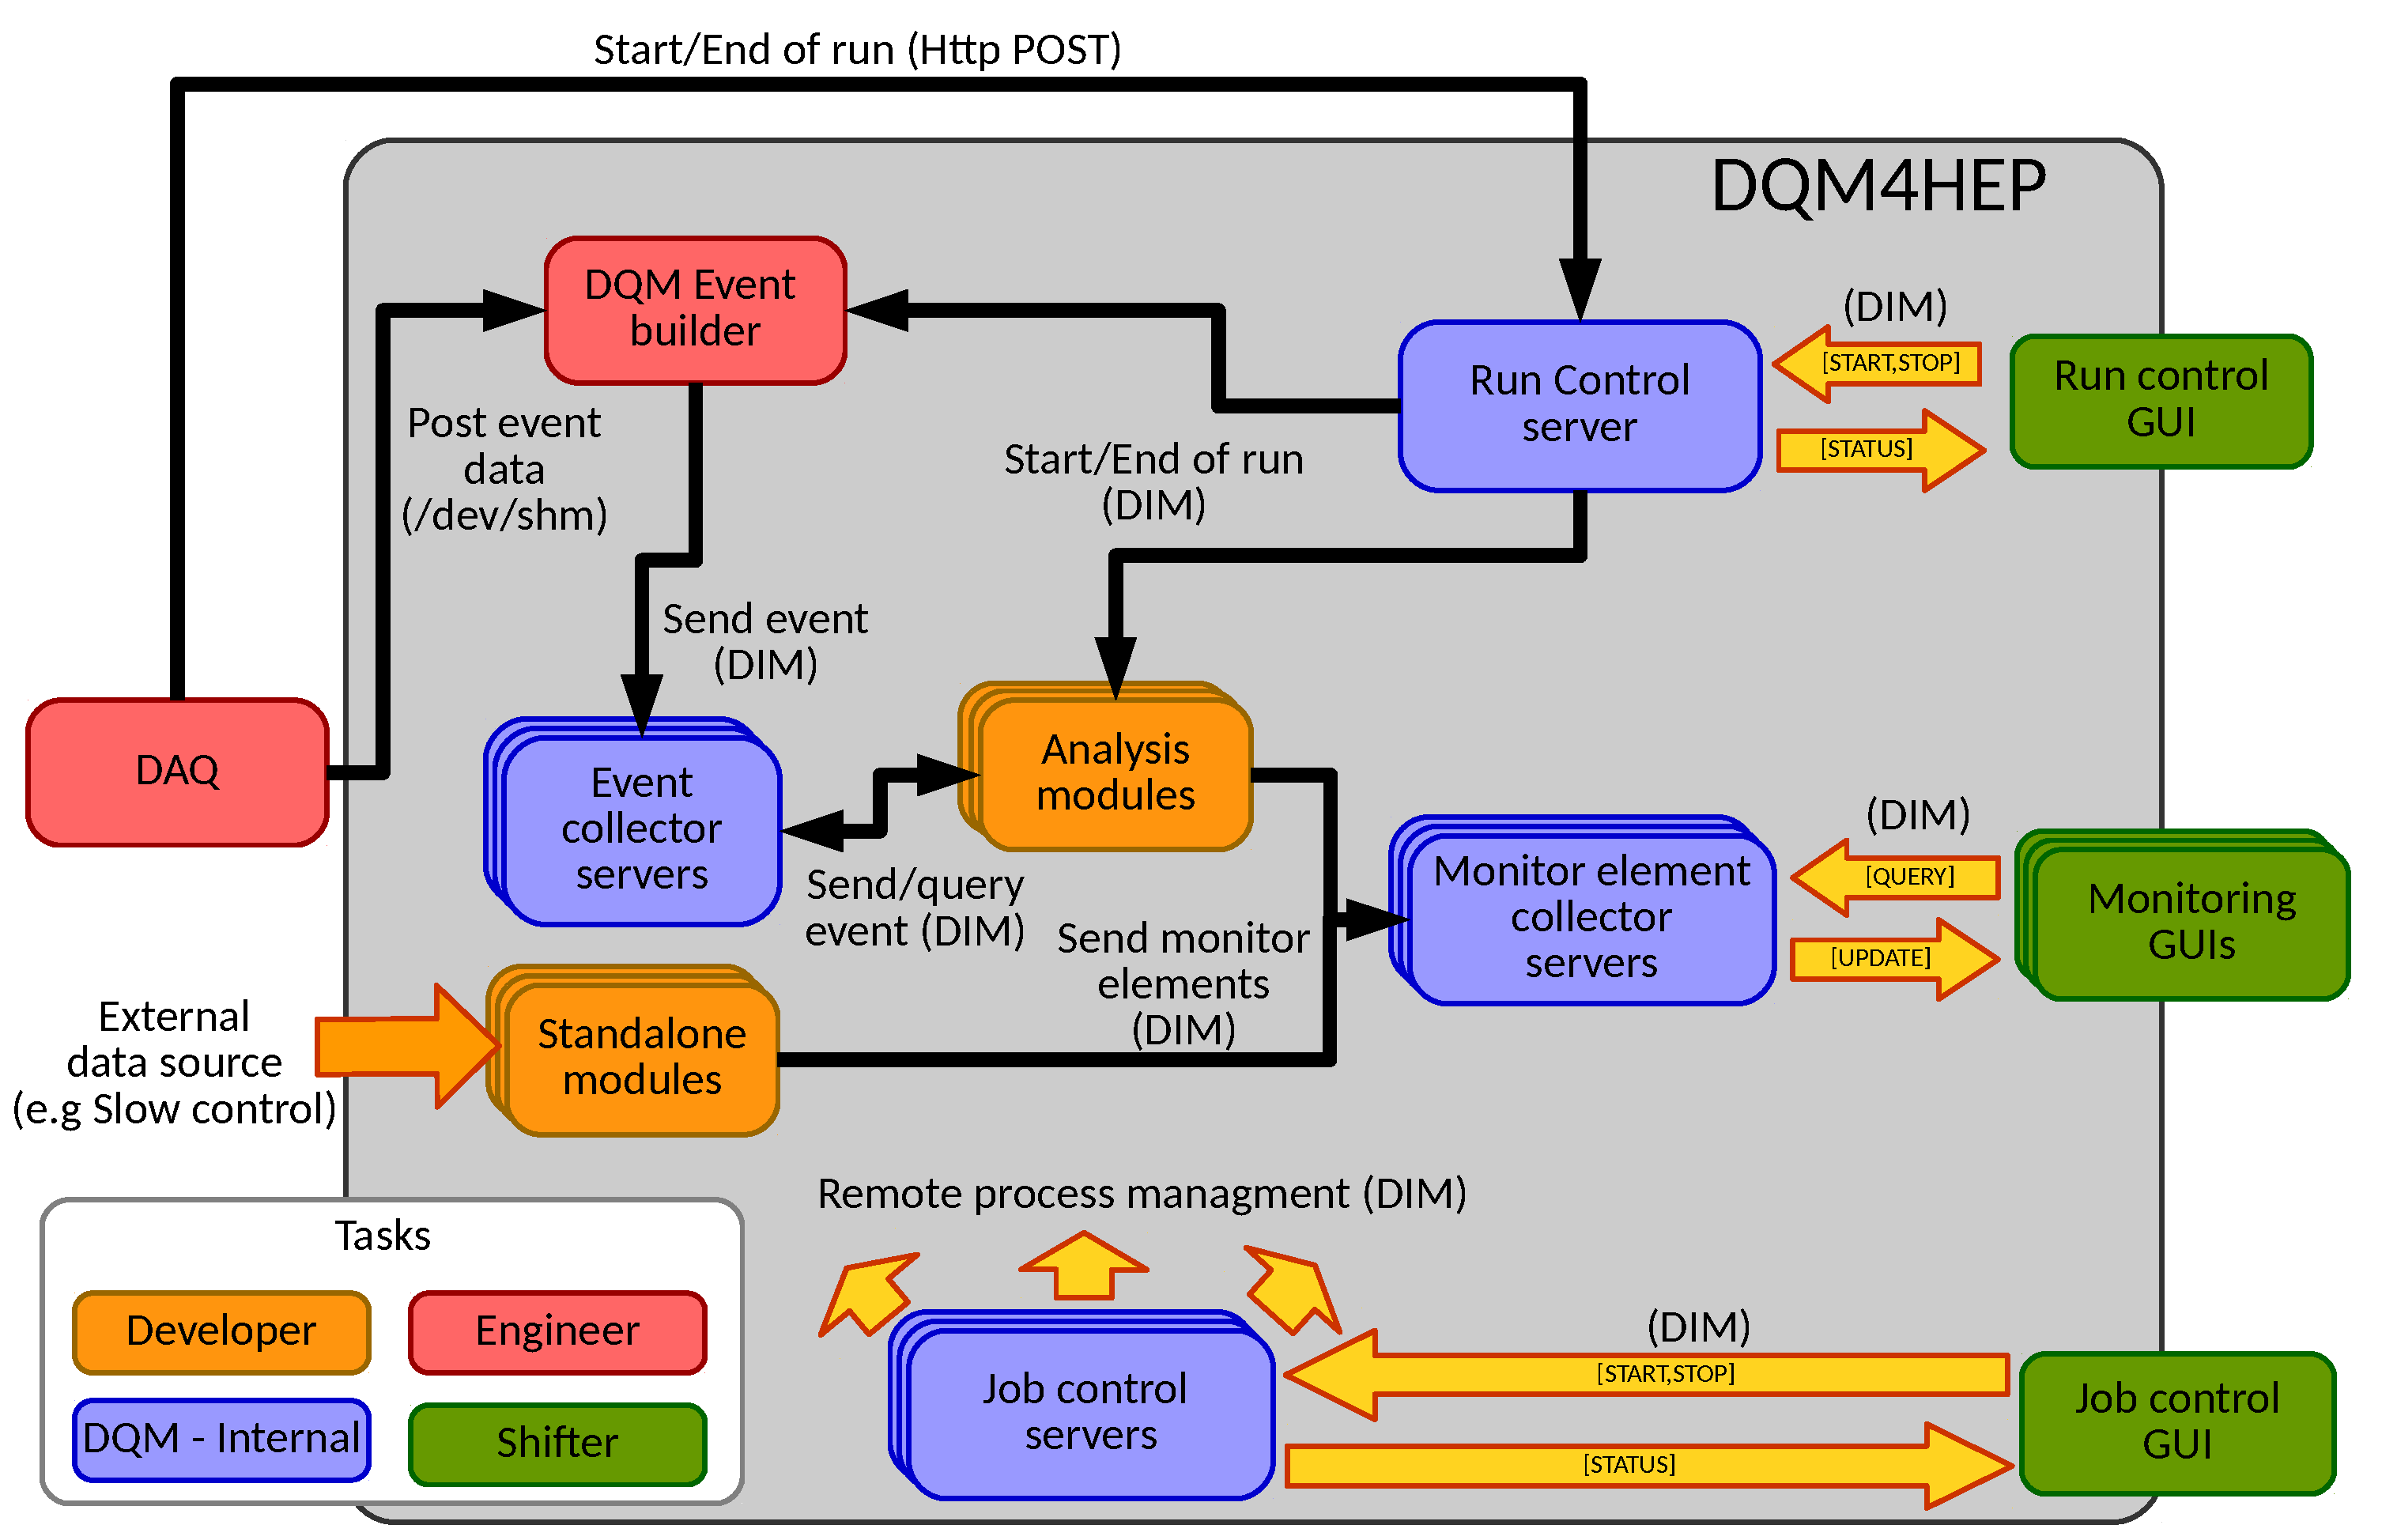
\includegraphics[width=0.95\linewidth]{figs/GlobalArchitectureDiagram.pdf}
    \caption{\label{fig:DQM4HEPArchitecture} DQM4HEP framework architecture.}
  \end{center}
\end{figure}


%~~~~~~~~~~~~~~~~~~~~~~~~~~~~~~~~~~~~~~~~~~~~~~~~~~~~~~~~~~~~~~~~%
\subsection{Link to DAQ system}
As explained before, to efficiently run an experiment, the monitoring system and the DAQ system have to be decoupled but the latter must send the data to the former in order to process them. To control the data acquisition, the DAQ system sends start/stop/status signals to the read out electronics of the detectors. The monitoring system can be set up to receive such signals by
its \textit{Run Control Server} before dispatching it to the DQM applications. Thus, starting (stopping) a new run from the DAQ system will automatically start (stop) the DQM applications.

Second coupling to the DAQ system is the \textit{event builder} as depicted in Fig.~\ref{fig:DQMEventBuilder}. Its purposes is to get the raw data collected by the DAQ system (e.g. from a shared memory space) and convert it to an user defined data structure using plugins called \textit{shm processors}. The reconstructed events are then serialized and sent to event collectors over the network.

\begin{figure}[htbp]
  \begin{center}
    \includegraphics[width=0.95\linewidth]{figs/EventBuilderDiagram_IEEE.pdf}
    \caption{\label{fig:DQMEventBuilder} Sketch of the event building process within the framework.}
  \end{center}
\end{figure}

It should be emphasized here that this is the only coupling to the DAQ system, and so represents the only work required from the DAQ engineer to couple the framework with an experiment.


%~~~~~~~~~~~~~~~~~~~~~~~~~~~~~~~~~~~~~~~~~~~~~~~~~~~~~~~~~~~~~~~~%
\subsection{Collectors}
With the ability of balancing the load over multiple cores and computers comes the need of a common access point for data. Two types of applications serve this process in the framework. The \textit{event collector} acts as the bridge between the event builder and the various analysis modules. The \textit{monitor element collector} share the same role between the analysis modules and the visualization interfaces.

As can be seen on Fig.~\ref{fig:DQMDataAccess}, data from the event collectors can then be accessed either via direct user query (i.e. modules send a query to the collector to receive the last recorded event) or via a subscription system (collectors notify modules when a new event is collected and send it).

To start such an application, only the collector name is needed. This name is set using command line argument at start-up and will be used to identify the collector over the network for external applications.

\begin{figure}[htbp]
  \begin{center}
    \includegraphics[width=0.95\linewidth]{figs/EventCollectorDiagram.pdf}
    \caption{\label{fig:DQMDataAccess} Schematic view of possible interactions between an event collector and a client application.}
  \end{center}
\end{figure}

%~~~~~~~~~~~~~~~~~~~~~~~~~~~~~~~~~~~~~~~~~~~~~~~~~~~~~~~~~~~~~~~~%
\subsection{Online data analysis}
Depending on the data input, two types of applications can be used within the framework. The first one, the analysis module, use reconstructed event from the event collectors and thus runs only while the DAQ is taking data. The second type, the standalone module, is independent of the DAQ status and use external data source defined by the user (e.g. environmental data stored in a database). The later runs until the user stop it.

Both are implemented as user defined plug-ins and aim to analyze and reduce data to a few self-described objects called \emph{monitor elements}. They wrap graphics objects such as histogram or graph, plus some meta data about data quality or run-time information.

Multiple quality tests can run on each monitor element to assess the data quality. Their results are bound to the monitor element and sent together to the collector so that user can then be alerted if quality reaches low/dangerous threshold (e.g. high current value, saturation in part of detector, etc.). If deemed necessary, user has the ability to archive monitor elements for off-line checks in ROOT \cite{ROOT} files.

The framework architecture gives the flexibility to start and stop any analysis modules at any given time, including during data taking. This important point means that adding, removing, modifying a module even while taking data will never interfere with DAQ system.

%~~~~~~~~~~~~~~~~~~~~~~~~~~~~~~~~~~~~~~~~~~~~~~~~~~~~~~~~~~~~~~~~%
\subsection{Cycle structure for data processing}

During a run, data taking can be non continuous or with a high rate. For performance reasons and logic, there is no need to refresh the visualization after each processed event. Thus, data are processed within a cycle structure, during which events are processed sequentially. At the end of a cycle, the monitor elements are sent to the collectors and the visualization interfaces are refreshed. Cycles are implemented as plug-ins so user can defined their own to suit their needs. The DQM4HEP framework provides three built-in cycle implementations :

\begin{itemize}
  \item a \textit{timer cycle}, for which events are processed during \textit{n} seconds,
  \item an \textit{event counter cycle}, for which \textit{n} events are processed before ending,
  \item an \textit{event size cycle}, for which \textit{n} bytes of serialized data are processed before ending.
\end{itemize}

Fig.~\ref{fig:DQMCycleSystem} shows the analysis module application workflow where the central part is dedicated to the cycle logic (\textit{start}/\textit{processEvent}/\textit{end}).

\begin{figure}[htbp]
  \begin{center}
    \includegraphics[width=0.7\linewidth]{figs/AnalysisModuleApplicatonWorkflowDiagram.pdf}
    \caption{\label{fig:DQMCycleSystem} Analysis module application workflow also showing cycle logic.}
  \end{center}
\end{figure}

\subsection{Remote control of the framework's application}
To deploy the framework for a detector setup, multiple applications needs to run (collectors, analysis modules, etc.), sometimes over multiple computers to balance the load. There is thus a need for an easy way of controlling all of them. \textit{Job control servers} serves this purpose. They run as Linux daemons on every host involved in the deployment. They fork new processes on demand from a remote client interface and take care of their management. These interfaces can also be used to access processes information, such as their status or environment variables.

%~~~~~~~~~~~~~~~~~~~~~~~~~~~~~~~~~~~~~~~~~~~~~~~~~~~~~~~~~~~~~~~~%
%~~~~~~~~~~~~~~~~~~~~~~~~~~~~~~~~~~~~~~~~~~~~~~~~~~~~~~~~~~~~~~~~%
\section{Qt \cite{QT} graphical user interfaces (GUIs)}

\subsection{Monitoring GUI}

This graphical user interface implements a multiple client access to monitor element collectors available over the network. User can browse the \textit{monitor element collectors} content and build a selection of elements to display. The main interface, as shown in Fig.~\ref{fig:DQMMainViz}, displays on the left, the list of \textit{monitor element (ME)} the user just selected. These \textit{ME} can be displayed on the drawing section where a set of canvases are organized in a tab system. Every drawn \textit{ME} is interactive and can be manipulated according to the frontend used to display them (only ROOT~\cite{ROOT} is available for now).

\begin{figure*}[htbp]
  \begin{center}
    \includegraphics[width=.95\textwidth]{figs/MaintInterfaceGUI.pdf}
    \caption{\label{fig:DQMMainViz} Main window of the monitoring GUI.
    1. Option for manual/auto update.
    2. Monitor Elements (ME) organized in a tree-like structure
    3. List of displayed ME customizable via dedicated GUI with available ME (coming from analysis modules currently loaded)
    4. Drawing section for ME, can be organized in multiple tabs.
    5. Drawn ME are interactive, here ROOT[3] object that can be manipulated (zoom, change scale, fit, save, etc.)
    }
  \end{center}
\end{figure*}

\subsection{Job control GUI}

This GUI is a graphic implementation of multiple job server clients. Processes to run are loaded from a JSON configuration file and listed as shown on Fig.~\ref{fig:JobControlGUI}. User can then start/stop application on the various hosts using the interface but also monitor the process status by querying single process status or starting a timer that refreshes the interface automatically. When starting a process on a host, a log file is created on the job control server and can be accessed at any time form this graphical user interface.

\begin{figure*}[htbp]
  \begin{center}
    \includegraphics[width=.95\textwidth]{figs/JobControlInterface.pdf}
    \caption{\label{fig:JobControlGUI} Job interface main window. Applications are ordered by host.}
  \end{center}
\end{figure*}

\subsection{Run control GUI}

It implements a graphical client interface to a run control server. The run control server application is mostly designed to receive start and stop run signals from the DAQ and dispatch it to all listening DQM applications. Moreover, the GUI implementation can also steers these signals and display the current run status in case the deployment is run without a DAQ, like in an offline test mode.

%~~~~~~~~~~~~~~~~~~~~~~~~~~~~~~~~~~~~~~~~~~~~~~~~~~~~~~~~~~~~~~~~%
%~~~~~~~~~~~~~~~~~~~~~~~~~~~~~~~~~~~~~~~~~~~~~~~~~~~~~~~~~~~~~~~~%
\section{Implementation}

As the framework was developed within the CALICE-SDHCAL\footnote{Semi Digital Hadronic CALorimeter} Collaboration, a dedicated implementation has been produced in parallel for this prototype. It is based on the LCIO~\cite{LCIO} Event Data Model, and provides interfaces for event type definition and serialization in this format.


Concerning the link to the DAQ system, the run control commands are received through HTTP POST and dispatch to the rest of the framework with DIM. The event building is based on \textit{levbdim}, the event builder used by the DAQ system for first level data reconstruction. In the SDHCAL case, the DAQ dumps the raw data coming from the detector to a shared memory (\textit{shm}) space as data sources buffers. The framework pulls a copy of these buffers and converts them to a LCIO format suitable for analysis with the online event builder implemented as plugins.

As the LCIO EDM contains multiple data structures for different levels of data reconstruction, converters are provided to pass from one such structure to the other. This gives the ability to use off-line analysis into the monitoring system, leading to a better assessment of the overall data quality.

For testing purposes, an offline data reader is also included in this implementation. This allows us to run the framework on previously recorded data stored on disk. It is especially handy to configure the framework properly in advance for a test beam campaign. To keep conditions as close as possible to a real setup, it can be configured to simulate the timing structure of the raw data.

At the online analysis level, along with our own analysis development, we gathered already existing analysis code for this experiment and adapted it to plug it into the framework. Some of these modules are briefly discussed hereafter.

The \textit{Event Display} module allows for 2D and 3D visualization of the data in the detector. A 70GeV pion interacting in the SDHCAL as seen in the monitoring system is displayed in Fig.~\ref{fig:DQMEventDisplay}. A slow control module monitors the high voltages and current (see Fig.~\ref{fig:DQMCurrents}) in every part of the detector together with the ambient temperature and pressure. This module is critical, as too high values of current or high voltage can irremediably compromise the detector working order and thus the data quality. A module is evaluating the efficiency for each of the 50 chambers of the SDHCAL. Another module gives informations related to the beam configuration such as rates of incoming particles as seen by the detector.

\begin{figure}[htbp]
  \begin{center}
    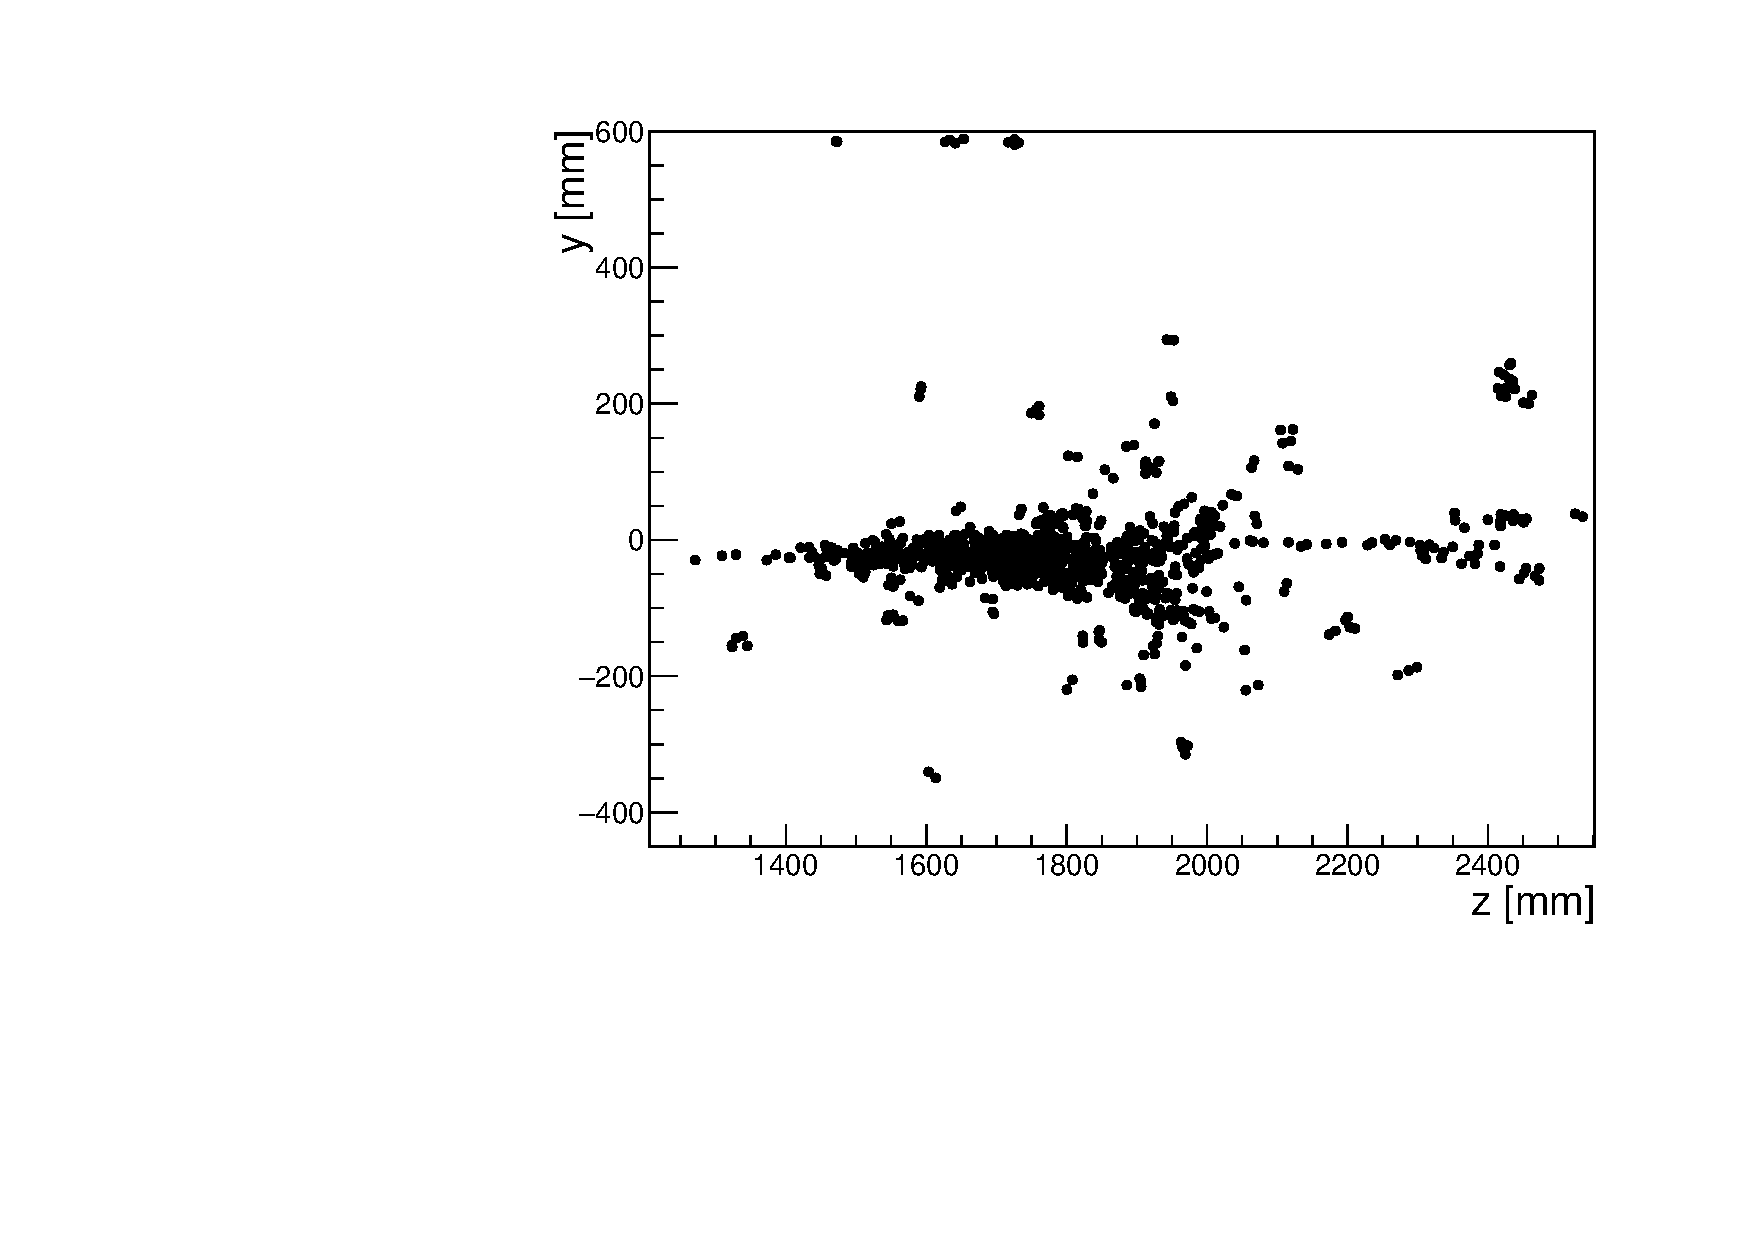
\includegraphics[width=0.95\linewidth]{figs/DQM_SDHCAL_Shower_pi-_70GeV_I732792.pdf}
    \caption{\label{fig:DQMEventDisplay} 2D Transversale view of a 70GeV pion in the SDHCAL prototype.}
  \end{center}
\end{figure}

\begin{figure}[htbp]
  \begin{center}
    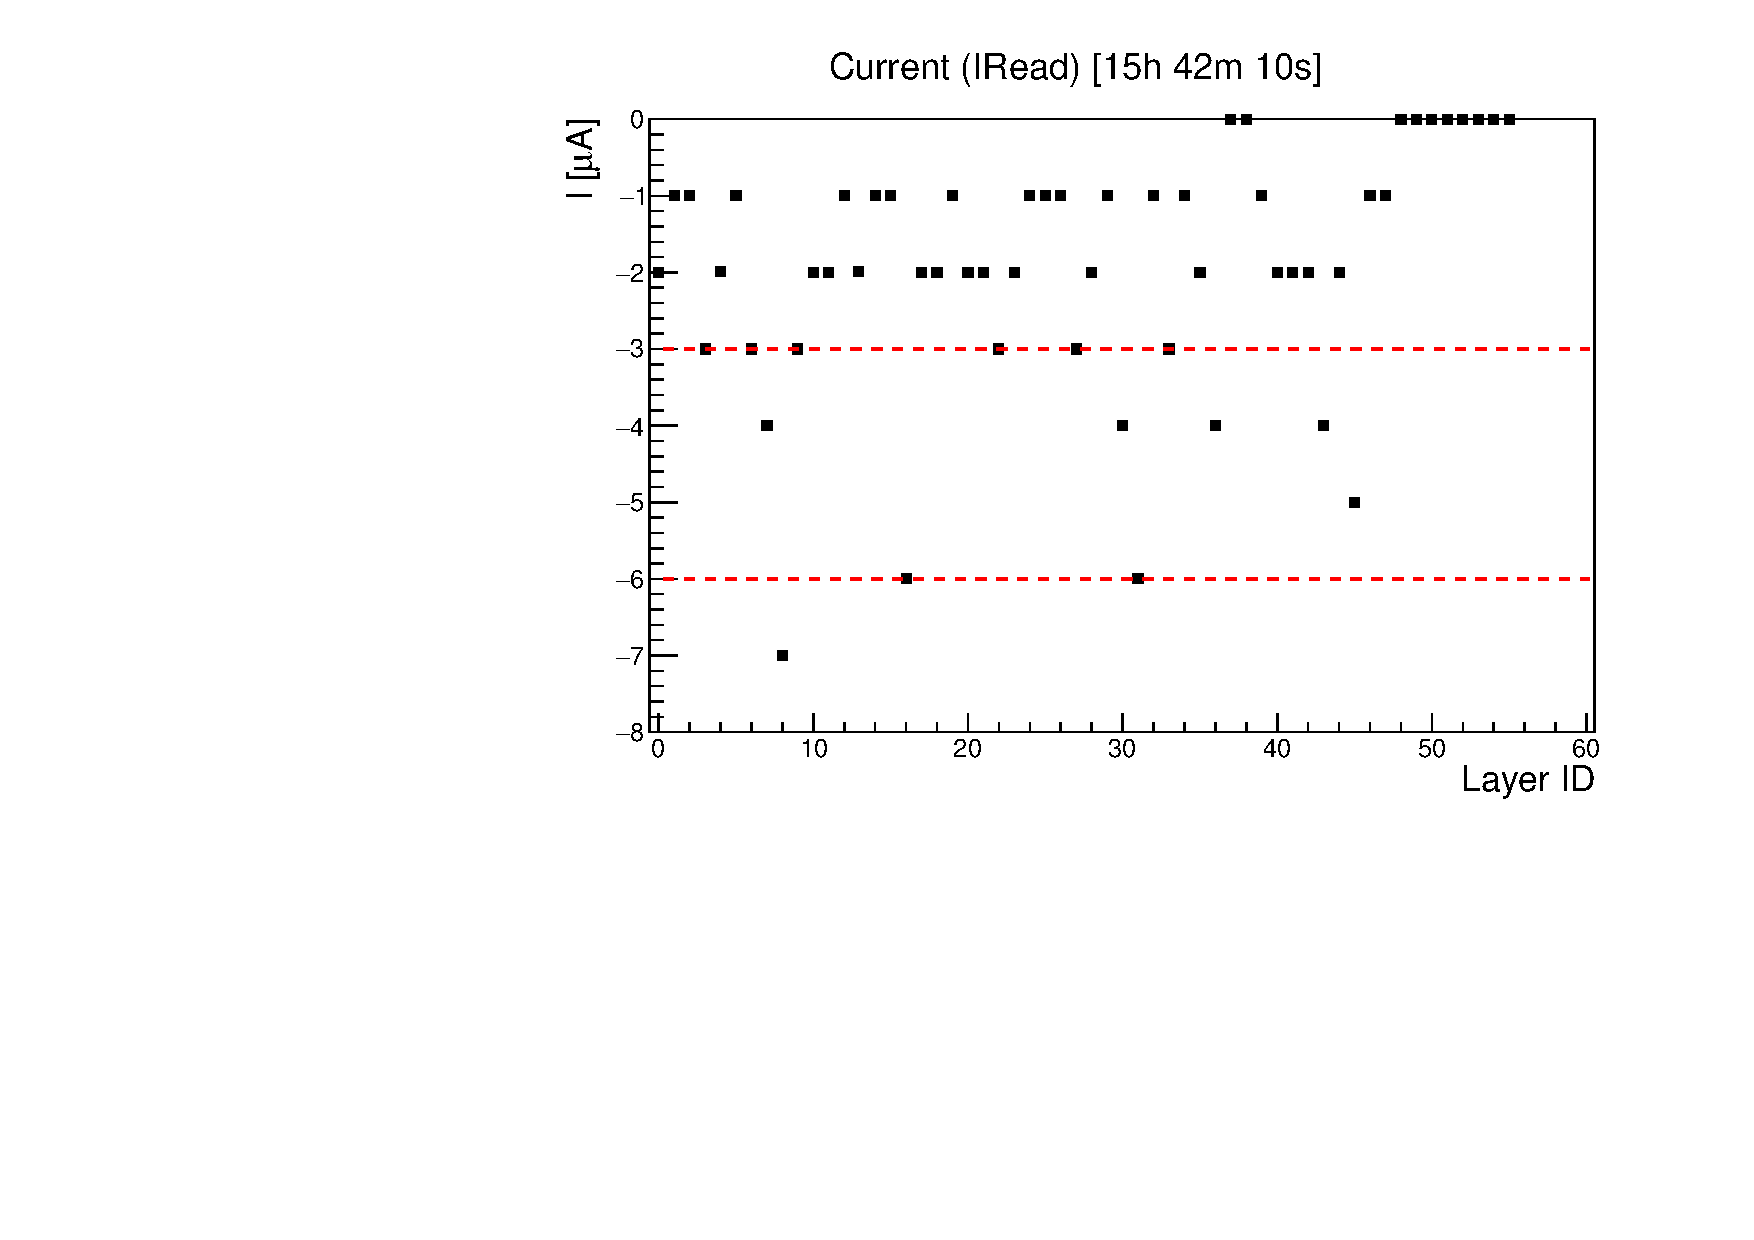
\includegraphics[width=0.95\linewidth]{figs/DQM_SDHCAL_Current_SC13.pdf}
    \caption{\label{fig:DQMCurrents} Instantaneous value for currents in SDHCAL prototype.}
  \end{center}
\end{figure}

One of these campaigns was dedicated to make a combined data taking with the CALICE-SiWEcal\footnote{Silicon (W)Tungsten Electronic calorimeter)} experiment. Thus, we also developed some analysis dedicated to monitoring parts of this prototype such as ADC counter maps for each detector layer as shown in  Fig.~\ref{fig:DQMEcalDisplay}).

\begin{figure}[htbp]
  \begin{center}
    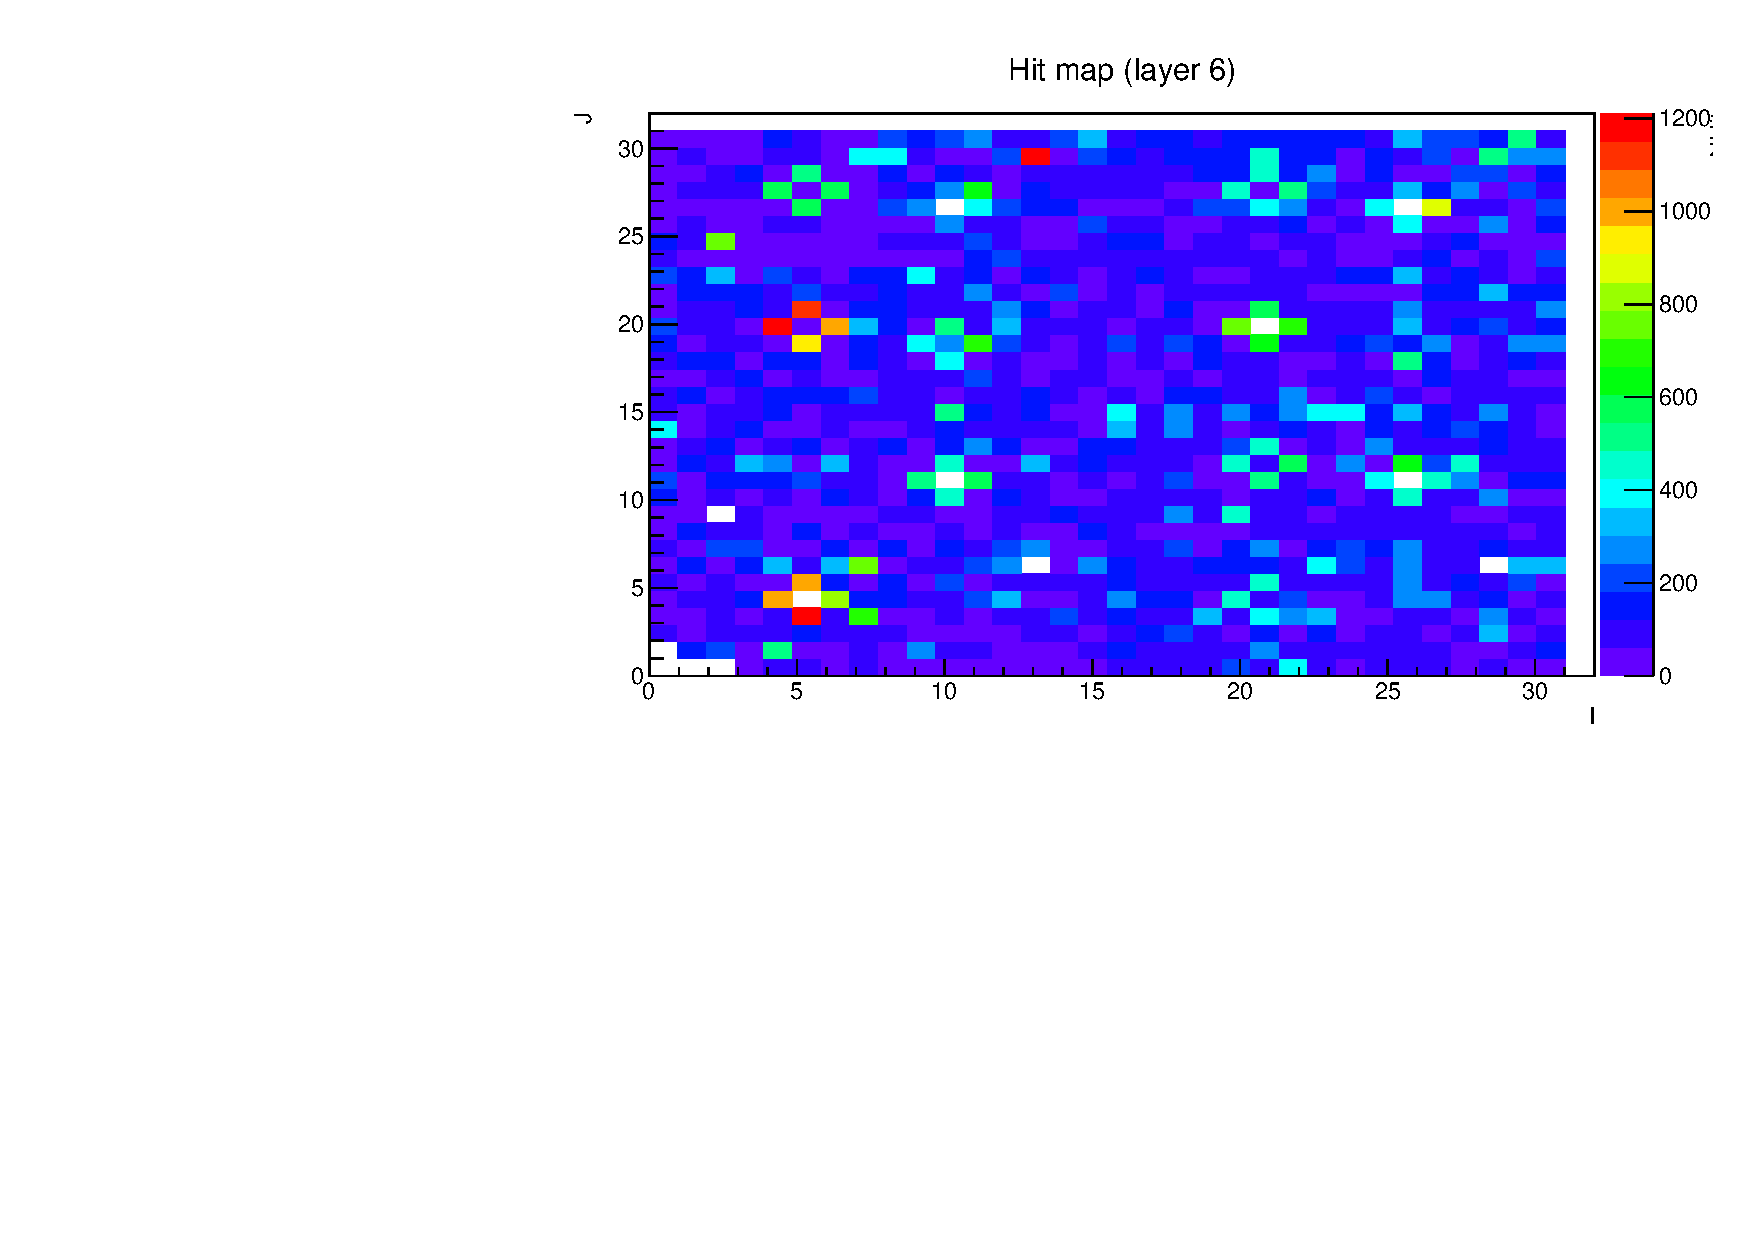
\includegraphics[width=\linewidth]{figs/DQM_SDHCAL_ECAL_HitMap6_I732891.pdf}
    \caption{\label{fig:DQMEcalDisplay} ADC counter map of layer 6 of the CALICE-SiWEcal during data taking in June 2016.}
  \end{center}
\end{figure}

With this deployment, shifters were able to quickly spot and correct problems including, but not limited to, bad gas circulation, undesirably noisy electronics, wrong beam configuration, etc...

%~~~~~~~~~~~~~~~~~~~~~~~~~~~~~~~~~~~~~~~~~~~~~~~~~~~~~~~~~~~~~~~~%
%~~~~~~~~~~~~~~~~~~~~~~~~~~~~~~~~~~~~~~~~~~~~~~~~~~~~~~~~~~~~~~~~%
\section{Conclusion}
In light of the critical importance of a tool to quickly detect problems and ensure a good data quality, a new generic framework for Data Quality Monitoring called DQM4HEP, was designed, integrating full flexibility across experiment setup.

In contrast with most systems available for High Energy Physics up to now, it is not tied to a given Event Data Model. All the tools needed to develop an experiment specific implementation, such as DAQ and serialization interface, data format and detector analysis, are provided within the framework. The whole system is written in c++11 with Qt~\cite{QT} libraries for the GUI.

The whole framework was tested both with offline and online setup dedicated to the SDHCAL prototype. The online configuration was used during two test beam campaigns at CERN. One of these campaign was a combined test with the CALICE-SiWEcal, for which online analysis were also developed in parallel and successfully deployed.


\IEEEtriggeratref{3}

\bibliographystyle{IEEEtran}


% references section

% can use a bibliography generated by BibTeX as a .bbl file
% BibTeX documentation can be easily obtained at:
% http://www.ctan.org/tex-archive/biblio/bibtex/contrib/doc/
% The IEEEtran BibTeX style support page is at:
% http://www.michaelshell.org/tex/ieeetran/bibtex/
%\bibliographystyle{IEEEtran}
% argument is your BibTeX string definitions and bibliography database(s)
%\bibliography{IEEEabrv,../bib/paper}
%
% <OR> manually copy in the resultant .bbl file
% set second argument of \begin to the number of references
% (used to reserve space for the reference number labels box)

\begin{thebibliography}{6}

\bibitem{LCIO}
% Frank Gaede, \emph{\tt lcio.desy.de}, 2016.
S. Aplin et al., "LCIO: A persistency framework and event data model for HEP", \emph{Nuclear Science Symp. and Medical Imaging Conf. (NSS/MIC), 2012 IEEE}, Anaheim, CA, 2012, pp. 2075-2079.

\bibitem{DIM}
C. Gaspar et al., "DIM, a Portable, Light Weight Package for Information Publishing, Data Transfer and Inter-process Communication" presented at the \emph{Int. Conf. Computing in High Energy and Nuclear Physics}, Padova, Italy, 2000)

\bibitem{MONGOOSE}
Michael J Hammel, "Mongoose: an embeddable web server in C", \emph{Linux Journal}, 2010, pp. 192

\bibitem{QT}
% J. Blanchette and M. Summerfield
Qt Company, \emph{\tt http://www.qt.io}, v4.7, 2016.

\bibitem{ROOT}
Rene Brun and Fons Rademakers, "ROOT - An Object Oriented Data Analysis Framework", \emph{Nucl. Inst. \& Meth. in Phys. Res. A 389}, 1997, pp. 81-86. Available: http://root.cern.ch/

\bibitem{MARLIN}
F. Gaede,  "Marlin and LCCD: Software tools for the ILC", \emph{Nucl. Inst. \& Meth. A559}, 2006, pp. 177-180

\end{thebibliography}






% that's all folks
\end{document}
